\documentclass[12pt]{article} 
\usepackage[margin=2cm]{geometry} 
\usepackage{psfrag} 
\usepackage{graphicx} 
\usepackage{epstopdf} 
\usepackage{longtable,booktabs} 
\usepackage{amsmath,amsfonts} 
\usepackage{breqn} 
\usepackage{float,morefloats,caption} 

\usepackage{mathtools} %% previously \usepackage{amsmath}
\usepackage{amsfonts}
\usepackage{amssymb} % http://www.ctan.org/tex-archive/macros/latex/required/psnfss/psnfss2e.pdf
%\usepackage[official]{eurosym}
\usepackage{helvet}
\usepackage{natbib}
\usepackage{lscape, longtable, array, booktabs, multirow, tabularx, graphics, epstopdf}
\usepackage{setspace}
\usepackage{listings}
\usepackage {tikz}
%\usepackage{listings}
%\usepackage{breqn}
%\usepackage{multicol}

\usepackage[lighttt]{lmodern}
\lstset{basicstyle=\ttfamily}
%\lstset{stringstyle=\normal}


\begin{document} 
\section*{Hansens' RBC model}
Please make sure you've read Uhlig's article, especially section 4. Take special note of: the timing convention; that $R_t$ is simply a definition; and, how to obtain the steady state.

\begin{equation}
\max E \sum^{\infty}_{t=0} \beta^{t} \left( \frac{C^{1-\eta}_t}{1-\eta} - A N_t   \right)
\end{equation}
s.t.
\begin{eqnarray} \label{resource}
C_t + I_t &=& Y_t \\ \label{law}
K_t &=& I_t + (1-\delta)K_{t-1}\\ \label{prodfunc}
Y_t &=& F(Z_t,K_{t-1},N_t) = Z_t K^{\rho}_{t-1} N^{1-\rho}_t \\ \label{techshock}
\log{Z}_t &=& (1-{\psi})\log{\bar{Z}} + {\psi}\log{Z}_{t-1} + \epsilon_t ~,~~ \epsilon_t \sim i.i.d.\mathcal{N}(0,\sigma^2)
\end{eqnarray}
We assume that \eqref{resource}, \eqref{law}, and \eqref{prodfunc} are binding.  \eqref{techshock} is exogenous and follows an AR(1) process, so we can ignore it; but this uncertainty necessitates the expectations operator in the FOCs for variables in $t+1$.
\begin{itemize}
\item Control variables: $K_t$; $N_t$ 
\item Endogenous state variables: $K_{t-1}$
\item Exogenous/Stochastic state variables: $Z_{t-1}$ 
\end{itemize}


\section{The value function}
Let $U(C_t,N_t) = \frac{C^{1-\eta}_t}{1-\eta} - {A}N_t$ be utility in period $t$. The value function follows:

\begin{eqnarray} \nonumber
V(K_{t-1},Z_{t-1}) &=& \max_{C_t,I_t,Y_t,K_t,N_t} U(C_t,N_t) + \beta E_t   \bigl[ V(K_{t},Z_{t})   \big] ~~ {\text{s.t.}}~  \eqref{resource}, \eqref{law}, \eqref{prodfunc}  \\ \nonumber
V(K_{t-1},Z_{t-1}) &=& \max_{C_t,I_t,Y_t,K_t,N_t} \left( \frac{C^{1-\eta}_t}{1-\eta} - A N_t   \right) + \beta E_t   \bigl[ V(K_{t},Z_{t})   \big] ~~ {\text{s.t.}}~  \eqref{resource}, \eqref{law}, \eqref{prodfunc}  \\ \nonumber
V(K_{t-1},Z_{t-1}) &=& \max_{I_t,Y_t,K_t,N_t} \left( \frac{(Y_t - I_t)^{1-\eta}}{1-\eta} - A N_t   \right) + \beta E_t   \bigl[ V(K_{t},Z_{t})   \big]  ~~ {\text{s.t.}}~  \eqref{law}, \eqref{prodfunc}  \\ \nonumber
V(K_{t-1},Z_{t-1}) &=& \max_{K_t,N_t} \left( \frac{(Z_t K^{\rho}_{t-1} N^{1-\rho}_t - K_t + (1-\delta)K_{t-1})^{1-\eta}}{1-\eta} - A N_t   \right) + \beta E_t   \bigl[ V(K_{t},Z_{t})   \big] 
\end{eqnarray}


\section{The first-order conditions}
Don't panic. You can use notation to save time and space. Let $\frac{\partial{U(\cdot)}}{\partial{C}} = U_c(\cdot) = C_t^{-\eta}$ be the marginal utility of consumption with respect to $C$. 

FOC $N_t$:
\begin{eqnarray} \nonumber
\frac{\partial V(\cdot_t)}{\partial N_t} &:& \frac{\partial U(C_t,N_t)}{\partial C_t}\frac{\partial C_t}{\partial Y_t}\frac{\partial Y_t}{\partial N_t} + \frac{\partial U(C_t,N_t)}{\partial N_t}= 0 ~~~~~~~~~~ \text{[chain rule]} \\ \nonumber
 && \frac{(1-\eta)C_t^{1-\eta -1}}{1-\eta}(1-\rho)Z_{t}K^{\rho}_{t-1}N_t^{1-\rho {\color{red}{- 1}}} - A = 0  \\ \nonumber
&& {C_t^{-\eta}}(1-\rho)Z_{t}K^{\rho}_{t-1}N_t^{1-\rho}{\frac{1}{\color{red}{N_t}}} - A = 0\\ \nonumber
\\ \label{FOCN}
\therefore & & A = {C_t^{-\eta}}(1-\rho){\frac{Y_t}{\color{red}{N_t}}} 
\end{eqnarray}
We can re-state \eqref{FOCN} as $$A{C_t^{\eta}} = (1-\rho)\frac{Y_t}{N_t}$$ which implies that the marginal rate of substitution between labour and consumption ($U_n/U_c$) equals the marginal product of labour $F_n(\cdot)$. \underline{Note: no envelope theorem needed (why?)}. \vskip0.25in

FOC $K_{t}$:

\begin{eqnarray} 
 \nonumber
\frac{\partial V(\cdot_t)}{\partial K_{t}} &:& \frac{\partial U(C_t,N_t)}{\partial C_t} \left[ \underset{=0}{\underbrace{\frac{\partial C_t}{\partial Y_t}\frac{\partial Y_t}{\partial K_{t}} }} + \frac{\partial C_t}{\partial I_t}\frac{\partial I_t}{\partial K_{t}}  \right] + \beta{E_t}\frac{\partial{V(\cdot_{t+1})}}{\partial{K_{t}}} = 0 ~~~~~~~~~~ \text{[chain rule]}  \\ \label{FOCK}  
&& C_{t}^{-\eta} (- 1)  + \beta{E_t}{\color{red}{\frac{\partial{V(\cdot_{t+1})}}{\partial{K_{t}}} }} = 0 
\end{eqnarray}

Envelope theorem:
\begin{eqnarray}
\frac{\partial{V(\cdot_{t})}}{\partial{K_{t-1}}} &:&  \frac{\partial U(C_t,N_t)}{\partial C_t} \left[ \frac{\partial C_t}{\partial Y_t}\frac{\partial Y_t}{\partial K_{t-1}} + \frac{\partial C_t}{\partial I_t}\frac{\partial I_t}{\partial K_{t-1}}  \right] + \underset{=0}{\underbrace{\beta{E_t}\frac{\partial{V(\cdot_{t+1})}}{\partial{K_{t-1}}}}} \\ 
&& C_{t}^{-\eta} \left[ \rho \frac{Z_{t}K_{t-1}^{\rho}N_t^{1-\rho}}{K_{t-1}} + (1-\delta) \right]   \\ 
&& C_{t}^{-\eta} [ \rho \frac{Y_t}{K_{t-1}} + (1-\delta) ]   
\end{eqnarray}
Iterate forward one period:
\begin{eqnarray} \label{FOCKenv}
{\color{red}{ \frac{\partial{V(\cdot_{t+1})}}{\partial{K_{t}}} }} &:& C_{t+1}^{-\eta} [ \rho \frac{Y_{t+1}}{K_{t}} + (1-\delta) ] = C_{t+1}^{-\eta} R_{t+1}  
\end{eqnarray}
Substitute \eqref{FOCKenv} into \eqref{FOCK} to get:
\begin{eqnarray} \nonumber
C_{t}^{-\eta} &=& \beta {E_t} \left[ C_{t+1}^{-\eta} R_{t+1} \right ]  \\ \label{Euler}
1 &=& \beta {E_t} \left[ \left(\frac{C_{t}}{C_{t+1}}\right)^{\eta} R_{t+1} \right ]
\end{eqnarray}
\eqref{Euler} gives the Euler equation which governs the intertemporal consumption path (and therefore capital).  In a competitive version of this model (i.e., market economy not social planner), this is an asset pricing equation by which the real return $R_t$ on an asset equates with the marginal product of capital (i.e., the return on investment in production). Note also that we assume certainty equivalence: $E[X Y] = E[X]E[Y]$, which implies that $cov[XY]=0$ (or is constant, since it will fall away after log-linearization). For small deviations from steady-state, a linear approximation is good. 


\section{Stead-states}
Obtain steady-states by dropping $t$ subscripts from FOCs and constraints and then simplify. Although there is know ``rule'' per se, some standard parameters are left to be calibrated (i.e., given values) and some are determined endogenously and some are substituted out completely (see sections 4 and 6 below). We are left with \textit{implied} three steady-state conditions (for the real rate of return, the physical capital stock to GDP ratio, and the consumption to GDP ratio) and five parameters to calibrate (excluding the size of the stochastic shock).

\begin{dmath*}
R = \frac{1}{{{\beta}}}
\end{dmath*}
\begin{dmath*}
\frac{K}{Y} = \frac{{{\rho}}}{{R}-\left(1-{{\delta}}\right)}
\end{dmath*}
\begin{dmath*}
\frac{C}{Y} = 1-{{\delta}}\, \frac{K}{Y}
\end{dmath*}


\section{System of log-linearized equations}
Follow the steps of Taylor and Uhlig to obtain the following log-linearized equations . [Hint: you will need to use the steady-state conditions to simplify the coefficients].

% Equation 1 resource constraint
\begin{dmath}
{{y}_{t}}=\frac{C}{Y}\, {{c}_{t}}+{{\delta}}\, \frac{K}{Y}\, {{v}_{t}}
\end{dmath}

% Equation 4 capital accumulation equation
\begin{dmath}
{{k}_{t}}=\left(1-{{\delta}}\right)\, {{k}_{t-1}}+{{\delta}}\, {{v}_{t}}
\end{dmath}

% Equation 5 production function
\begin{dmath}
{{y}_{t}}={{z}_{t}}+{{\rho}}\, {{k}_{t-1}} + {(1-\rho)}\,{{n}_{t}}
\end{dmath}


% Equation 6 TFP process
\begin{dmath}
{{z}_{t}}={{\psi}}\, {{z}_{t-1}}+{{\epsilon_z}_{t}}
\end{dmath}

% Equation 7 labour supply
\begin{dmath}
{{\eta}}\, {{c}_{t}} = {{y}_{t}} - {{n}_{t}}
\end{dmath}


% Equation 2 Euer equation
\begin{dmath}
0 = E_t[{{\eta}}\,({{c}_{t}} - {{c}_{t+1}})] + {{r}_{t+1}}
\end{dmath}

% Equation 3 return on capital
\begin{dmath}
{{r}_{t}}={{\rho}}\, \frac{Y}{{K}}\, \left({{y}_{t}}-{{k}_{t-1}}\right)
\end{dmath}



 


% \pagebreak

\section{Impulse response functions}

\begin{figure}[hpb]\centering \vskip-1in
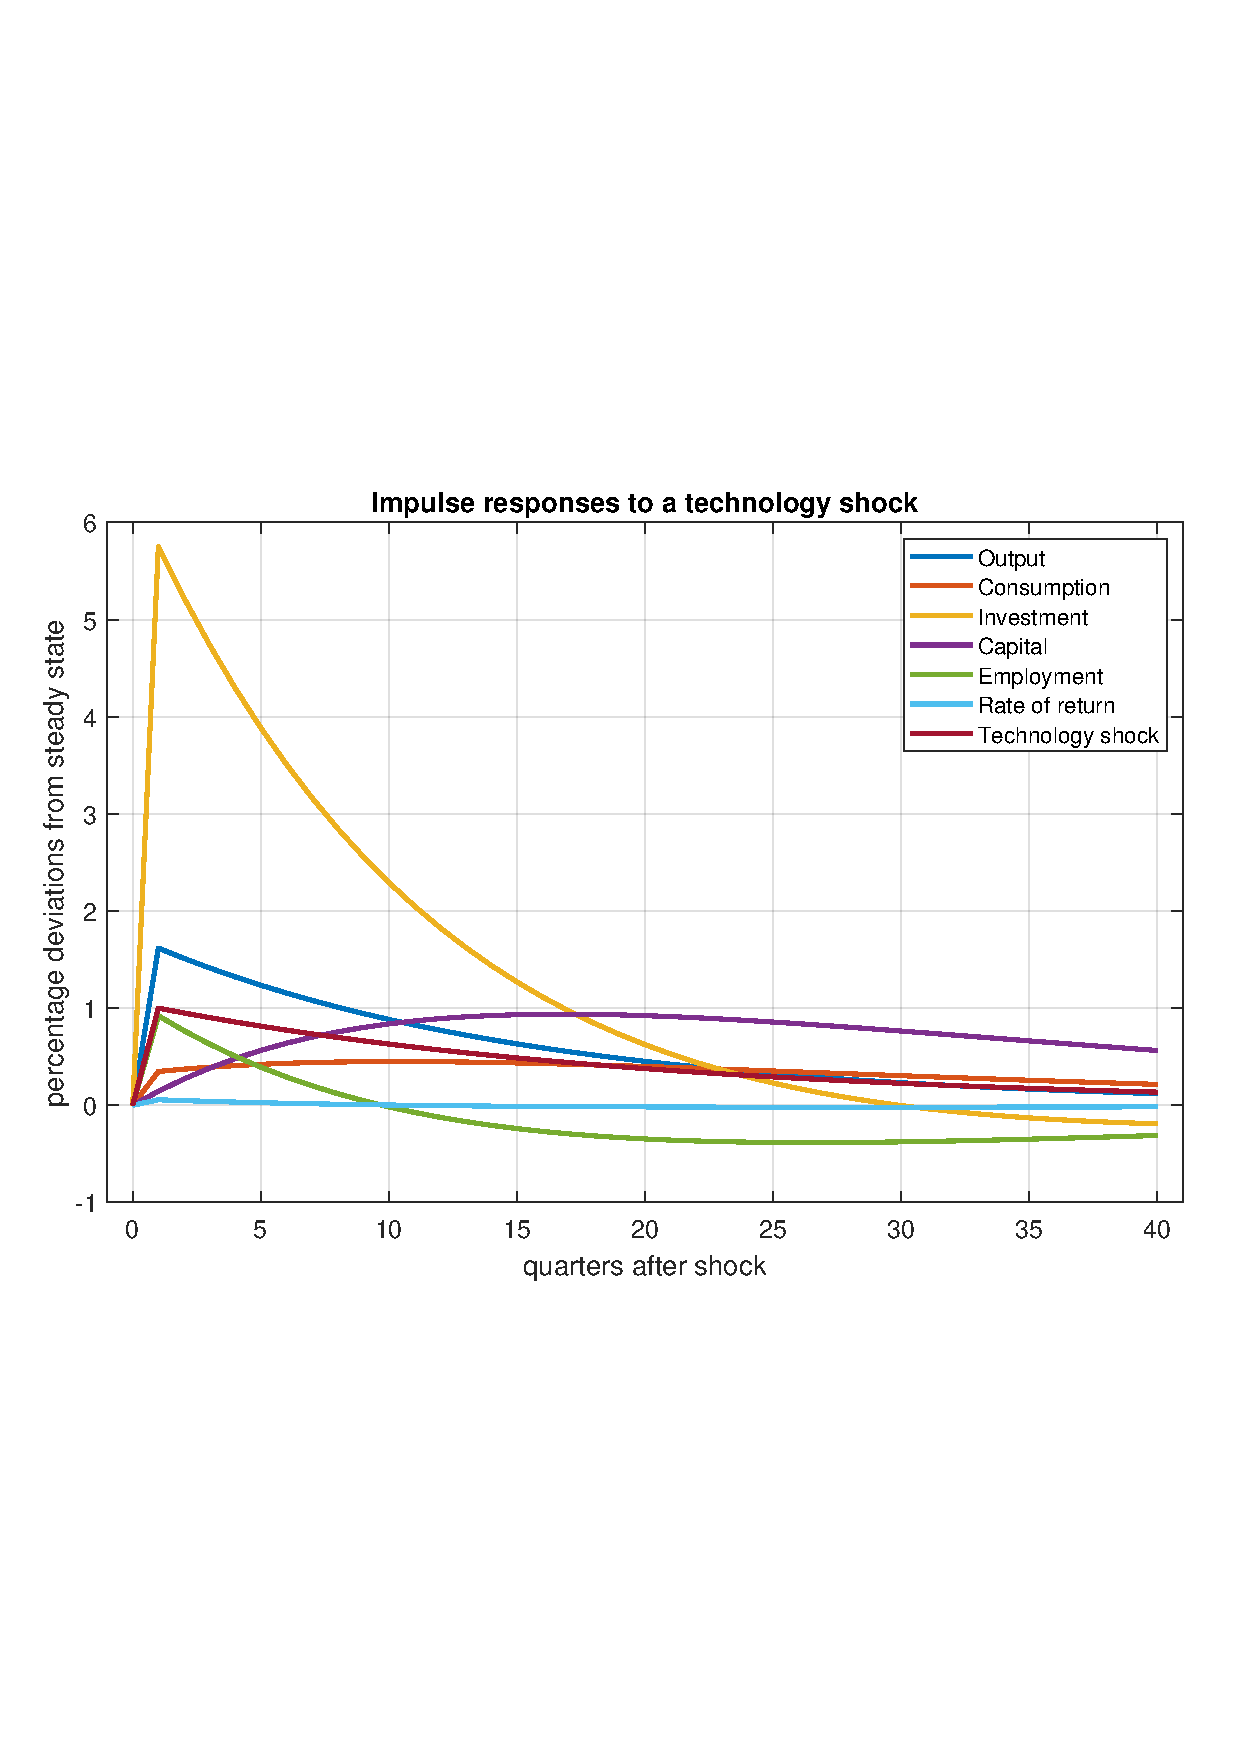
\includegraphics[width=0.75\textwidth]{basicrbc_fig.pdf}
\end{figure}


\section{\texttt{DYNARE} and \LaTeX ~definitions}
\nopagebreak

{\footnotesize
\begin{center}
\begin{longtable}{ccc}
\caption{Endogenous}\\%
\hline%
\multicolumn{1}{c}{\textbf{Variable}} &
\multicolumn{1}{c}{\textbf{\LaTeX}} &
\multicolumn{1}{c}{\textbf{Description}}\\%
\hline\hline%
\endfirsthead
\multicolumn{3}{c}{{\tablename} \thetable{} -- Continued}\\%
\hline%
\multicolumn{1}{c}{\textbf{Variable}} &
\multicolumn{1}{c}{\textbf{\LaTeX}} &
\multicolumn{1}{c}{\textbf{Description}}\\%
\hline\hline%
\endhead
\texttt{y} & ${y}$ & output\\
\texttt{c} & ${c}$ & consumption\\
\texttt{n} & ${n}$ & hours\\
\texttt{v} & ${v}$ & investment\\
\texttt{k} & ${k}$ & capital\\
\texttt{r} & ${r}$ & real rate\\
\texttt{z} & ${z}$ & TFP\\
\hline%
\end{longtable}
\end{center}
\begin{center}
\begin{longtable}{ccc}
\caption{Exogenous}\\%
\hline%
\multicolumn{1}{c}{\textbf{Shock}} &
\multicolumn{1}{c}{\textbf{\LaTeX}} &
\multicolumn{1}{c}{\textbf{Description}}\\%
\hline\hline%
\endfirsthead
\multicolumn{3}{c}{{\tablename} \thetable{} -- Continued}\\%
\hline%
\multicolumn{1}{c}{\textbf{Variable}} &
\multicolumn{1}{c}{\textbf{\LaTeX}} &
\multicolumn{1}{c}{\textbf{Description}}\\%
\hline\hline%
\endhead
\texttt{epsilon} & ${\epsilon_z}$ & TFP shock\\
\hline%
\end{longtable}
\end{center}
\begin{center}
\begin{longtable}{ccc}
\caption{Parameters}\\%
\hline%
\multicolumn{1}{c}{\textbf{Parameter}} &
\multicolumn{1}{c}{\textbf{\LaTeX}} &
\multicolumn{1}{c}{\textbf{Description}}\\%
\hline\hline%
\endfirsthead
\multicolumn{3}{c}{{\tablename} \thetable{} -- Continued}\\%
\hline%
\multicolumn{1}{c}{\textbf{Variable}} &
\multicolumn{1}{c}{\textbf{\LaTeX}} &
\multicolumn{1}{c}{\textbf{Description}}\\%
\hline\hline%
\endhead
\texttt{rho} & ${\rho}$ & capital share\\
\texttt{bet} & ${\beta}$ & discount factor\\
\texttt{delt} & ${\delta}$ & depreciation rate\\
\texttt{psi} & ${\psi}$ & persistence TFP shock\\
\texttt{eta} & ${\eta}$ & risk aversion\\
\texttt{sigmae} & ${\sigma_{e}}$ & i.i.d TFP shock\\
\hline%
\end{longtable}
\end{center}
 
%\begin{center}
\begin{longtable}{ccc}
\caption{Parameter Values}\\%
\toprule%
\multicolumn{1}{c}{\textbf{Parameter}} &
\multicolumn{1}{c}{\textbf{Value}} &
 \multicolumn{1}{c}{\textbf{Description}}\\%
\midrule%
\endfirsthead
\multicolumn{3}{c}{{\tablename} \thetable{} -- Continued}\\%
\midrule%
\multicolumn{1}{c}{\textbf{Parameter}} &
\multicolumn{1}{c}{\textbf{Value}} &
  \multicolumn{1}{c}{\textbf{Description}}\\%
\midrule%
\endhead
${\rho}$ 	 & 	 0.330 	 & 	 capital share\\
${\beta}$ 	 & 	 0.990 	 & 	 discount factor\\
${\delta}$ 	 & 	 0.025 	 & 	 depreciation rate\\
${\psi}$ 	 & 	 0.950 	 & 	 persistence TFP shock\\
${\eta}$ 	 & 	 5.000 	 & 	 risk aversion\\
${\sigma_{e}}$ 	 & 	 0.010 	 & 	 i.i.d TFP shock\\
\bottomrule%
\end{longtable}
\end{center}
 
}


\section{The full \texttt{DYNARE} \texttt{.mod} file}

\nopagebreak
{\footnotesize
\lstinputlisting{basicrbc2015binder.mod}
% [language=Matlab]
}




\end{document} 
